\documentclass{article}
\usepackage{graphicx}
\usepackage{color}
\usepackage{bm}
\usepackage{amsmath}

\sloppy
\definecolor{lightgray}{gray}{0.5}
\setlength{\parindent}{24pt}

\begin{document}

    \title{Pendulum Coding Problem}    
    \author{Johnathan Corbin\\Spaceflight Mechanics - Spring 2019}   
    \date{\today}
    \maketitle
\pagebreak

\tableofcontents
\pagebreak

\section{Formula Derivation}

\begin{figure}[h]
\centering
\includegraphics[width=1\textwidth]{figure1}
\caption{Simple Planar Pendulum System}
\label{figure1}
\end{figure}

	Figure \ref{figure1} is a diagram of a simple planar pendulum system. The pendulum swings in the plane of $\hat{n_1}$ and $\hat{n_2}$. In this case, we will consider the rod to have no mass and as having a negligible width, so as not to experience any drag forces. In addition, the rod is of a constant length $L = 2.0 meters$ from point \textit{O}. The sphere has a mass $m = 0.04kg$ and a radius of $r = 0.05 meters$.
	
	The reference frame $\hat{n_1}$ and $\hat{n_2}$ is taken to be adequately inertial for the purposes of this problem. The entire system is acted upon by standard gravity \textit{g} that acts in the direction shown in figure \ref{figure1}. The room has an atmosphere $\rho = 1.2250 \frac{kg}{m^3}$ and the mass has a coefficient of drag $c_d = 0.42$ that will be used in the calculation of the drag force acting on the mass. 

\begin{figure}[h]
\centering
\includegraphics[width=1\textwidth]{FreeBody}
\caption{Free Body Diagram of Mass m}
\label{FreeBody}
\end{figure}

\pagebreak

	Analysis of this problem begins with the free body diagram shown in figure \ref{FreeBody}. Newton's second law provides a good starting point and is given by:
	\begin{equation}
	\sum \vec{F}^{\,m} = m\vec{a}
	\end{equation}
Using the free body diagram, it can be shown that for this system, Newton's second law becomes the following:
	\begin{equation}
	\sum \vec{F}^{\,m} = m\vec{a} = T\hat{a_2}-mg\hat{n_2}+F_d\hat{a_1}
	\end{equation}
	Inspection of figure \ref{figure1} shows that the motion of the mass is restricted to rotating about point \textit{O} at a constant radius of \textit{L}. If we assume that point \textit{O} is fixed and in an intertial frame, then the acceleration $\vec{a}$ of \textit{m} is given by the following equation:
	\begin{equation}
	\vec{a}=(\ddot{L} - L\dot{\theta}^2)\hat{e_r} + (L\ddot{\theta} + 2\dot{L}\dot{\theta})\hat{e_\theta}
	\end{equation}
	In our case, \textit{L} is a constant value. As such, $\dot{L} = 0$ and $\ddot{L} = 0$. Additionally, we need to remember that $\hat{a_2} = -\hat{e_r}$ and $\hat{a_1} = \hat{e_\theta}$. Substituting these into equation (3) results in the following definition for the forces on mass \textit{m}:
	\begin{equation}
	\sum \vec{F}^{\,m} = m\vec{a} = T\hat{a_2}-mg\hat{n_2}+F_d\hat{a_1} = m(L\ddot{\theta}\hat{a_1} + L\ddot{\theta}^2\hat{a_2})
	\end{equation}
	
	We now have a single vector equation to describe the acceleration of the mass. From this vector equation, we can determine two scalar equations, one for $\hat{a_1}$ and another for $\hat{a_2}$. First, it is necessary for us to define the value for the drag force, $F_d$, and to also convert the $\hat{n_2}$ basis in our motion equation into the $\hat{a_1}$ and $\hat{a_2}$ basis. 	

\begin{figure}[h]
\centering
\includegraphics[width=1\textwidth]{Basis}
\caption{Basis Transform for $\hat{n_2}$}
\label{Basis}
\end{figure}

Using figure \ref{Basis} as a guide, one can determine that $\hat{n_2} = sin(\theta)\hat{a_1} + cos(\theta)\hat{a_2}$. Additionally, $F_d = \frac{\rho\dot{\theta}^2c_dA(-sign(\theta))}{2}$ where \textit{A} is the frontal area of the mass and the $(-sign(\theta))$ function is essential to ensuring that the drag force acts to always oppose the direction of velocity, even if the velocity changes signs. Without this term, the drag force would always act in the same $\hat{a_1}$ direction, causing the velocity to increase for half the time and subsequently slow the mass down for the other half. In reality, the drag is always working to slow the mass. Once these two additions are taken into account, the equation of motion can be split into the following two scalar equations:
	\begin{equation}
	\hat{a_1}: mL\ddot{\theta} = F_d - mgsin(\theta)
	\end{equation}
	\begin{equation}
	\hat{a_2}: mL\dot{\theta}^2 = T - mgcos(\theta)
	\end{equation}
For this problem, we are interested in the motion of the mass, not the tension force in the rod. As such, equation (6) can be safely discarded. Equation (5) is more useful for our analysis and will be used for the rest of the derivations to determine the motion of the mass. Substituting the previous equation for $F_d$ into equation (5) yields the following:
	\begin{equation}
	\boxed{\ddot{\theta} + \frac{sign(\dot{\theta})\rho c_d L \dot{\theta}^2A}{2m} + \frac{gsin(\theta)}{L}=0}
	\end{equation}
	
	Equation (7) is our full nonlinear equation of motion for the mass. To solve this equation analytically, several assumptions need to be made to simplify the system. In our case, we will assume that $c_d = 0$ in order to remove the drag force term and also that at small angles, $sin(\theta)\approx \theta$. After these approximations, our system becomes the following: 
	\begin{equation}
	\ddot{\theta} + \frac{g\theta}{L} = 0
	\end{equation}
To analytically solve this system, we start by finding the characteristic equation and then finding the roots $r_1$ and $r_2$. The characteristic equation is given by the following:
	\begin{equation}
	r^2 + \frac{g}{L} = 0
	\end{equation}
From the characteristic equation, it can be found that there are two complex roots: $r_1 = \sqrt{\frac{g}{L}}i$ and $r_2 = -\sqrt{\frac{g}{L}}i$. If the complex roots of the characteristic equation are of the form $r_{1,2} = \lambda\pm\mu i$, then the general solution to the differential equation is as follows: 
	\begin{equation}
	\theta(t) = c_1e^{\lambda t}cos(\mu t)+c_2e^{\lambda t}sin(\mu t)
	\end{equation}
In our case, $\mu=\sqrt{\frac{g}{L}}$ and $\lambda = 0$. The unknowns $c_1$ and $c_2$ will be determined from the given initial conditions for the system. The problem specifies two separate sets of initial conditions for us to consider. The first set of initial conditions is $[\theta_0, \dot{\theta_0}] = [75deg, 0]$ and the second set is $[\theta_0, \dot{\theta_0}] = [170deg, 0]$. Prior to finding the unknown constants, our general solution is of the form:
	\begin{equation}
\theta(t) = c_1cos(\sqrt{\frac{g}{L}} t)+c_2sin(\sqrt{\frac{g}{L}}t)
\end{equation}

\subsection{Analytic Approach}

\subsubsection{75 Degree Displacement}

At $t = 0$, we have the following initial conditions: $[\theta_0, \dot{\theta_0}] = [75deg, 0]$. Substituting these values into equation (11) and the derivative of equation (11) results in two equations with two unknowns. From this system of equations one can determine that $c_1 = 75 deg = \frac{5\pi}{12} rad$ and $c_2 = 0$. This results in the following analytic solution for an initial displacement of 75 degrees: 
	\begin{equation}
	\theta(t) = \frac{5\pi}{12}cos(\sqrt{\frac{g}{L}})
\end{equation}	 

\subsubsection{170 Degree Displacement}

At $t = 0$, we have the following initial conditions: $[\theta_0, \dot{\theta_0}] = [170deg, 0]$. Substituting these values into equation (11) and the derivative of equation (11) results in two equations with two unknowns. From this system of equations one can determine that $c_1 = 170 deg = \frac{17\pi}{18} rad$ and $c_2 = 0$. This results in the following analytic solution for an initial displacement of 170 degrees: 
	\begin{equation}
	\theta(t) = \frac{17\pi}{18}cos(\sqrt{\frac{g}{L}})
\end{equation}

\subsection{Numerical Approach}
From figures \ref{75} and \ref{170} it is apparent that the analytic results previously acquired were only accurate within a limited range. To improve our results, we need to adjust the simplifications that were made to the system. Previously we had assumed that $c_d = 0$ and $sin(\theta)\approx \theta$. If we now consider the effects of drag and disregard the small angle approximation, we will have a more accurate model of our system, but it becomes significantly harder to find an analytic answer for. The next two sections will look at how removing these two assumptions and solving the systems numerically can improve the accuracy of our results.

To numerically solve the new equations of motion, the ode45 function in Matlab will be utilized. All code used in this report can be found in the Matlab Code portion (section \ref{Code}).

\subsubsection{Without Aerodynamic Drag}
\label{aeroNoDrag}
In this section, the effects of the small angle approximation are going to be examined. We will still assume that $c_d = 0$ for now. By removing the small angle approximation, our new equation of motion is as follows:
	\begin{equation}
	\boxed{\ddot{\theta} + \frac{gsin(\theta)}{L} = 0}
	\end{equation}
Section \ref{75nodrag} contains the code used to analyze equation (14) for an initial displacement of 75 degrees. Section \ref{170nodrag} contains the code used to analyze equation (14) for an initial displacement of 170 degrees. In addition, both methods utilized the function in section \ref{noDrag} to supply $ode45$ with the proper time derivatives. The results for both can be seen in figures \ref{75} and \ref{170}.

\subsubsection{With Aerodynamic Drag}
In section \ref{aeroNoDrag} we examined how the small angle approximation affects the accuracy of our results. Now, let's examine how the addition of a drag force can get us closer to an accurate model of the system. As previously stated, we are going to assume that $c_d = 0.42$ for the mass. After accounting for drag, our new equation of motion is as follows:
\begin{equation}
\boxed{\ddot{\theta} + \frac{sign(\dot{\theta})\rho c_d L \dot{\theta}^2 A}{2m}+\frac{gsin(\theta)}{L}=0}
\end{equation}
For equation (15) it is important to note the $sign(\dot{\theta})$ function in the drag term. Without this function, the drag will not oppose the velocity of the mass at all times. Matlab has a built-in function for $sign()$. The $sign(\dot{\theta})$ function can be described as working as follows:
\begin{equation}
sign(\dot{\theta}) =
\begin{cases}
-1, & \dot{\theta} < 0 \\
0, & \dot{\theta} = 0 \\
1, & \dot{\theta} > 0 \\
\end{cases}
\end{equation}
Section \ref{75drag} contains the code used to analyze equation (15) for an initial displacement of 75 degrees. Section \ref{170drag} contains the code used to analyze equation (15) for an initial displacement of 170 degrees. In addition, both methods utilized the function in section \ref{drag} to supply $ode45$ with the proper time derivatives. The results for both can be seen in figures \ref{75} and \ref{170}.

\section{Results}
Figures \ref{75} and \ref{170} are graphs showing the results from all three different methods of analysis. The legend accompanying each graph distinguishes which results belong to the analytic result, numerical without drag, and numerical with drag.

Upon inspection, it is apparent that early in the time scale at 75 degrees, all three methods give very similar answers that start to lose accuracy around the 2 second mark. However, for 170 degrees, the analytic result gives a very poor estimate of the position of the mass. This result is expected and is a consequence of the small angle approximation we made in order to simplify the system. The larger the angle that we input into our analytic response, the worse the small angle approximation we made becomes. This is why we see such a poor approximation of the position for the large initial angle of 170 degrees in the analytic result.

In addition to the error resulting from the small angle approximation, we can see that in the numerical result that accounts for drag is slowly dampened over time. The drag force that opposes the velocity of the mass is what is responsible for slowing the motion of the mass. In the analytic result, we neglected drag altogether, which is why the system appears to oscillate forever without slowing down. The same is true of the numerical result we determined for the system with no drag. The only difference between the two is the phase of the oscillations. 

In reality, the mass obviously will not oscillate forever. As such, our analytic result and numerical result with no drag are poor approximations of how the system truly behaves. They are only accurate on very small time scales, when the drag force hasn't had enough time to significantly slow the mass. As such, the analytic response is really only valuable for showing which variables affect the system and how they can be changed to achieve different results from the system. If we wanted to determine the position of the mass after a long position of time, we would instead use the numerical result that incorporated drag, rather than the analytic result. 

\begin{figure}[h]
\centering
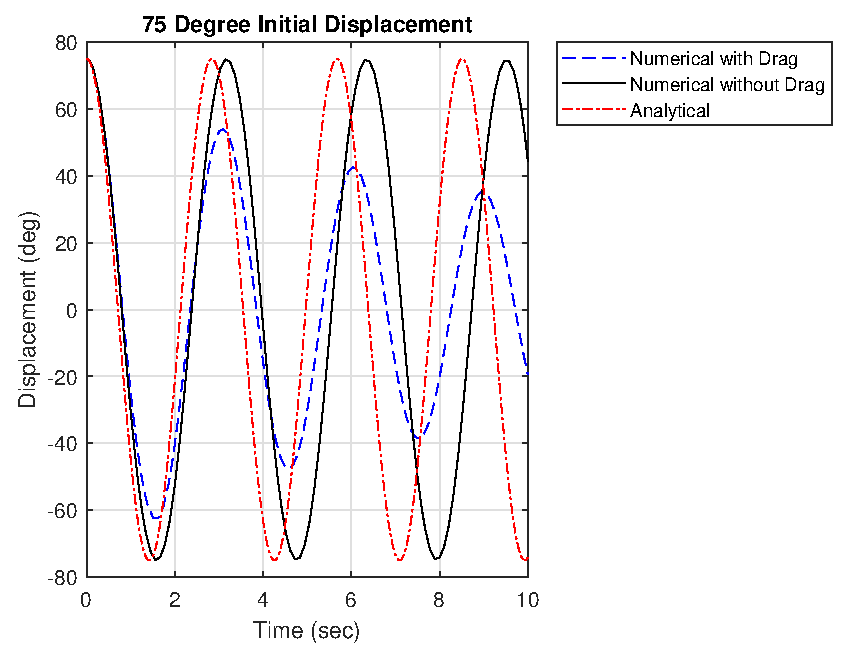
\includegraphics[width=1\textwidth]{Pendulum_03.eps}
\caption{Plots of the Analytic and Numerical Results for 75 Degree Displacement}
\label{75}
\end{figure}
\pagebreak

\begin{figure}[h]
\centering
\includegraphics[width=1\textwidth]{Pendulum_06.eps}
\caption{Plots of the Analytic and Numerical Results for 170 Degree Displacement}
\label{170}
\end{figure}

\pagebreak
\section{Matlab Code}
\label{Code}

\subsection{Main}

\begin{verbatim}
clear, clc

global L m g rho drag_coefficient interval area

%Declaring constants
L = 2; %length of rod [meters]
m = .04; %mass of sphere [kg]
radius = .05; %radius of sphere [m]
g = 9.81; %acceleration due to gravity [m/s^2]
rho = 1.225; %density of air [kg/m^3]
drag_coefficient = .42; %coefficient of drag
interval = [0,10]; %time interval [s]

area = pi * radius^2; %frontal area of sphere [m^2]
\end{verbatim}


\subsubsection{75 Degree Displacement - Numerical with Drag}
\label{75drag}

\begin{verbatim}
initial_conditions = [75 * pi / 180; 0]; %initial conditions [deg deg/s]

fname = 'PendulumFuncDrag'; %Setting name of the .m file for the state
%variable time derivatives

[time, y] = ode45(fname, interval, initial_conditions);

figure(1)
plot(time, y(:,1) * 180 / pi, '--b');
ylabel('Displacement (deg)')
xlabel('Time (sec)')
hold on
grid on
\end{verbatim}



\subsubsection{75 Degree Displacement - Numerical without Drag}
\label{75nodrag}

\begin{verbatim}
fname = 'PendulumFunc';

[time, y] = ode45(fname, interval, initial_conditions);

plot(time, y(:,1) * 180 / pi, 'k');
\end{verbatim}



\subsubsection{75 Degree Displacement - Analytical}

\begin{verbatim}
time = 0:.01:10; %time interval (sec)
theta0 = 75 * pi / 180;

theta = theta0 * cos(sqrt(g / L) * time);

plot(time, theta * 180 / pi, '-.r')
legend('Numerical with Drag', 'Numerical without Drag', 'Analytical',...
    'Location', 'bestoutside')
title('75 Degree Initial Displacement')
\end{verbatim}

\subsubsection{170 Degree Displacement - Numerical with Drag}
\label{170drag}

\begin{verbatim}
initial_conditions = [170 * pi / 180; 0]; %initial conditions [deg deg/s]

fname = 'PendulumFuncDrag'; %Setting name of the .m file for the state
%variable time derivatives

[time, y] = ode45(fname, interval, initial_conditions);

figure(2)
plot(time, y(:,1) * 180 / pi, '--b');
ylabel('Displacement (deg)')
xlabel('Time (sec)')
hold on
grid on
\end{verbatim}



\subsubsection{170 Degree Displacement - Numerical without Drag}
\label{170nodrag}

\begin{verbatim}
fname = 'PendulumFunc';

[time, y] = ode45(fname, interval, initial_conditions);

plot(time, y(:,1) * 180 / pi, 'k');
\end{verbatim}



\subsubsection{170 Degree Displacement - Analytical}

\begin{verbatim}
time = 0:.01:10; %time interval (sec)
theta0 = 170 * pi / 180;

theta = theta0 * cos(sqrt(g / L) * time);

plot(time, theta * 180 / pi, '-.r')
legend('Numerical with Drag', 'Numerical without Drag', 'Analytical',...
    'Location', 'bestoutside')
title('170 Degree Initial Displacement')
\end{verbatim}


\subsection{Functions}
\subsubsection{Numerical - No Drag}
\label{noDrag}

 \begin{verbatim}
 function dydt = PendulumFunc(t, y)
% Program determine the first order time derivatives of variable vector y = [y1,y2] for
% the current values of y and time t.
global L g
 % can be easily used by the the dydt script

 dydt = zeros(size(y)); % initialize to zero and makes column vector

 dydt(1) = y(2);

 dydt(2) = -(g * sin(y(1))) / L;
\end{verbatim}

\subsubsection{Numerical - Drag}
\label{drag}

 \begin{verbatim}
 function dydt = PendulumFuncDrag(t, y)
% Program determine the first order time derivatives of variable vector y = [y1,y2] for
% the current values of y and time t.
global L m g rho drag_coefficient area
 % can be easily used by the the dydt script

 dydt = zeros(size(y)); % initialize to zero and makes column vector

 dydt(1) = y(2);

 dydt(2) = (-sign(y(2)) * rho * L * drag_coefficient * y(2)^2 * area) / (2 * m) - (g * sin(y(1))) / L;
\end{verbatim}



\end{document}
    
